\section{Results}
\subsection{Recovery across occlusion and spacing}
Table~\ref{tab:main} gives every condition. At 20~mm, reconstruction raised fruit pixel recall at every branch count: from 68\% to 94\% with three branches, 49\% to 87\% with four, 42\% to 87\% with five, and 25\% to 42\% with six. It kept precision at 77--82\%. Count F1 rose by a similar margin: 0.62 to 0.79, 0.56 to 0.76, 0.42 to 0.77 and 0.14 to 0.55. At six branches, recovery is only partial. Just 14 of 27 views passed alignment validation, and whole clusters are missing (Fig.~\ref{fig:qual}); the reference view's own mask had 41\% precision there, which consensus raised to 77\%.

Wider spacing helped only under light occlusion. With three branches, 40~mm gave the best count F1 (0.88; its 25 detections hide three misses offset by three false positives, which is why we match detections rather than compare totals). With four or more branches, wider spacing lost recall, and losses track view rejection. At five branches and 40~mm, only 8 of 14 views survived, and both recall and F1 fell to the single-view level. At six branches and 60~mm, 3 of 9 views survived, recall fell below the single view, and GrapeSAM detected nothing.

\begin{table}[t]
\centering
\caption{Main results with SAM~3 masks. Views are those kept after alignment validation. Fruit-pixel recall $R$, precision $P$ and IoU are for the reconstruction, with the occluded reference view's recall as $R_\text{single}$. Count F1 is GrapeSAM against 25 labels, and $n$ is its number of detections on the reconstruction. Single-view precision is 85, 81, 86 and 41\% for 3--6 branches.}
\label{tab:main}
\scriptsize
\setlength{\tabcolsep}{3.6pt}
\begin{tabular}{@{}ccc cccc ccc@{}}
\toprule
 & & & \multicolumn{4}{c}{Fruit pixels (\%)} & \multicolumn{3}{c}{GrapeSAM count}\\
\cmidrule(lr){4-7}\cmidrule(lr){8-10}
Br. & mm & Views & $R_\text{single}$ & $R$ & $P$ & IoU & $F1_\text{single}$ & $F1$ & $n$\\
\midrule
3 & 20 & 28/28 & 68 & 94 & 80 & 0.76 & 0.62 & 0.79 & 36\\
3 & 40 & 14/14 & 68 & 92 & 86 & 0.80 & 0.62 & 0.88 & 25\\
3 & 60 & 9/9 & 68 & 88 & 90 & 0.80 & 0.62 & 0.83 & 23\\
\addlinespace[1pt]
4 & 20 & 28/28 & 49 & 87 & 80 & 0.72 & 0.56 & 0.76 & 30\\
4 & 40 & 14/14 & 49 & 74 & 84 & 0.65 & 0.56 & 0.72 & 22\\
4 & 60 & 7/9 & 49 & 52 & 89 & 0.49 & 0.56 & 0.54 & 12\\
\addlinespace[1pt]
5 & 20 & 28/28 & 42 & 87 & 82 & 0.73 & 0.42 & 0.77 & 27\\
5 & 40 & 8/14 & 42 & 42 & 91 & 0.40 & 0.42 & 0.39 & 6\\
5 & 60 & 9/9 & 42 & 57 & 93 & 0.54 & 0.42 & 0.48 & 8\\
\addlinespace[1pt]
6 & 20 & 14/27 & 25 & 42 & 77 & 0.38 & 0.14 & 0.55 & 15\\
6 & 40 & 8/13 & 25 & 27 & 87 & 0.26 & 0.14 & 0.28 & 4\\
6 & 60 & 3/9 & 25 & 9 & 80 & 0.08 & 0.14 & 0.00 & 0\\
\bottomrule
\end{tabular}
\end{table}

\begin{figure*}[t]
\centering
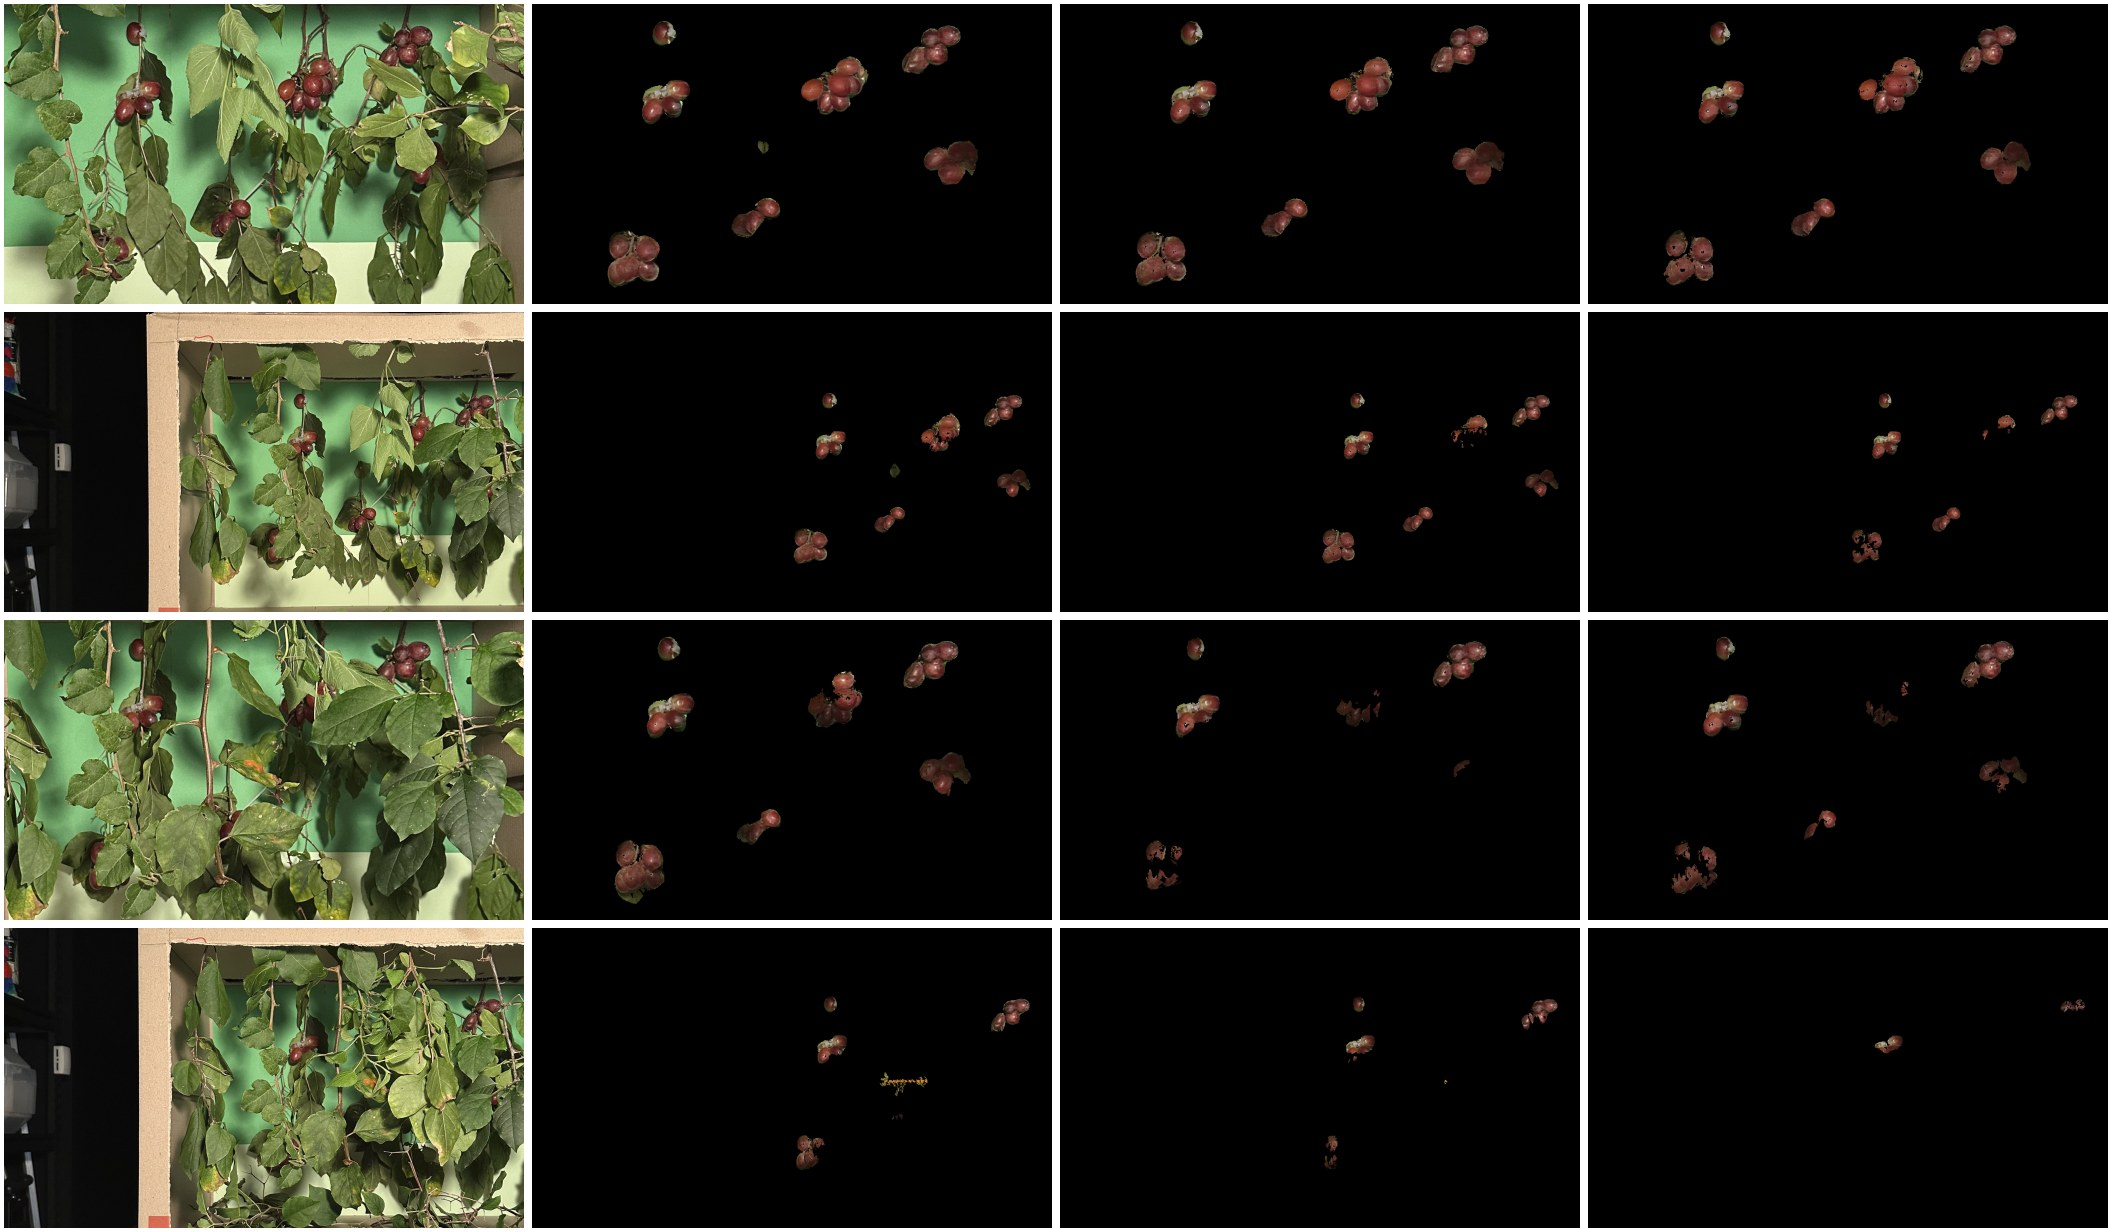
\includegraphics[width=0.42\textwidth]{figures/qualitative_grid.jpg}
\caption{Qualitative results. Rows show 3--6 foreground branches. Columns show the occluded reference view, then reconstructions at 20, 40 and 60~mm spacing, all cropped to the same fruit region. Black means no observation-backed fruit. Clusters disappear as spacing widens under heavy occlusion. At six branches, a strip of stem passed through the masks at 20~mm, and almost nothing survived at 60~mm.}
\label{fig:qual}
\end{figure*}

\subsection{Comparison with baselines}
Table~\ref{tab:baselines} compares fusion rules on the same views. Alignment is the larger factor. Depth-shift synthetic aperture, our prototype, gave count F1 of 0.72 to 0.78 at three branches; the mean and median collapsed to 0.08 at five branches, and all three statistics to 0.00 at six. Switching the same statistics to our feature-based alignment recovered much of the loss for the median (0.54 to 0.68, 0.08 to 0.44 and 0.00 to 0.33 at four to six branches) and the masked mean. The plain mean stayed poor, because foliage still contaminates it. Among the fusion rules, mask union had the highest recall (94--95\% up to five branches) but a precision of only 59--66\%. Mask majority had the opposite profile, with only 22\% recall at five branches. Our consensus rule combined 87\% recall with 80--82\% precision at four and five branches. Every other rule was at least six points lower in recall or in precision. It also had the best or equal-best count F1 at five and six branches. At three branches, the aligned median (0.84) and mask union (0.83) counted slightly better than ours (0.79). At four, the aligned masked mean was level with ours (0.78 against 0.76). These differences are similar in size to the effect of shifting the truth registration by 5~px (up to 0.08 F1), so we do not read them as a ranking.

\begin{table*}[t]
\centering
\caption{Fusion baselines at 20~mm, all using SAM~3 masks and the same views. $R$ and $P$ are fruit-pixel recall and precision (\%), and F1 is the GrapeSAM count F1. SA is synthetic aperture~\cite{vaish2006}. ``Depth shift'' is our prototype's alignment, and ``our alignment'' uses the poses of Sec.~\ref{sec:registration}. SA outputs are segmented by running SAM~3 on the fused image.}
\label{tab:baselines}
\scriptsize
\begin{tabular}{@{}lcccccccccccc@{}}
\toprule
Method & \multicolumn{3}{c}{3 branches} & \multicolumn{3}{c}{4 branches} & \multicolumn{3}{c}{5 branches} & \multicolumn{3}{c}{6 branches}\\
\cmidrule(lr){2-4}\cmidrule(lr){5-7}\cmidrule(lr){8-10}\cmidrule(lr){11-13}
 & R & P & F1 & R & P & F1 & R & P & F1 & R & P & F1\\
\midrule
Single view & 68 & 85 & 0.62 & 49 & 81 & 0.56 & 42 & 86 & 0.42 & 25 & 41 & 0.14\\
\addlinespace[2pt]
Mask union & 95 & 66 & 0.83 & 94 & 59 & 0.76 & 94 & 63 & 0.73 & 60 & 41 & 0.55\\
Mask majority & 75 & 97 & 0.72 & 46 & 95 & 0.48 & 22 & 92 & 0.21 & 14 & 83 & 0.21\\
\addlinespace[2pt]
SA mean, depth shift & 85 & 88 & 0.72 & 76 & 79 & 0.21 & 65 & 83 & 0.08 & 0 & 0 & 0.00\\
SA median, depth shift & 83 & 89 & 0.72 & 71 & 76 & 0.54 & 50 & 88 & 0.08 & 0 & 0 & 0.00\\
SA masked mean, depth shift & 95 & 65 & 0.78 & 95 & 56 & 0.55 & 93 & 60 & 0.50 & 0 & 0 & 0.00\\
\addlinespace[2pt]
SA mean, our alignment & 87 & 87 & 0.56 & 74 & 77 & 0.31 & 80 & 76 & 0.25 & 45 & 73 & 0.00\\
SA median, our alignment & 90 & 85 & 0.84 & 71 & 85 & 0.68 & 53 & 89 & 0.44 & 28 & 73 & 0.33\\
SA masked mean, our alignment & 95 & 76 & 0.79 & 94 & 64 & 0.78 & 89 & 70 & 0.72 & 61 & 65 & 0.41\\
\addlinespace[2pt]
Ours & 94 & 80 & 0.79 & 87 & 80 & 0.76 & 87 & 82 & 0.77 & 42 & 77 & 0.55\\
\bottomrule
\end{tabular}
\end{table*}

\subsection{Ablations}\label{sec:ablation}
Table~\ref{tab:ablation} varies one component at a time at five branches. \textbf{Colour consensus is what keeps the output countable.} Without it, pixel recall and precision barely changed (89\% and 80\%), but count F1 fell from 0.77 to 0.26. Removing every consensus rule gave 94\% recall but an F1 of 0.30. Pixel metrics alone would rate these variants as good as the full method. We attribute the drop, without testing it directly, to colour copied from inconsistent sources breaking up berry appearance.

\textbf{Minimum views} trades recall for precision. Raising $m$ from 1 to 3 raised precision from 63\% to 82\% with no loss in count F1, but $m=5$ cost 10 points of recall and reduced F1 to 0.67. \textbf{The minimum span} had no effect up to 40~mm, because at 20~mm spacing any three distinct views already span 40~mm. The rule matters only for denser sampling, such as video, and 80~mm removed real fruit. Copying versus blending the output colour made no measurable difference.

\textbf{Fruit-only features are essential.} With SIFT on the whole image, fewer than three views passed validation and no reconstruction was produced. Colour masks in place of SAM~3 lost 21 points of recall. The joint solve and held-out check did not matter here, because no view was rejected at five branches. Chained similarities and a translation-only model did equally well, although translation-only raised the median held-out error from 0.68 to 1.04~px. A homography overfitted (F1 0.59), and the foliage mask had no measurable effect.

\begin{table}[t]
\centering
\caption{Ablations at five branches and 20~mm. Fusion and mask variants reuse the full method's poses. Values are fruit-pixel recall and precision (\%) and GrapeSAM count F1.}
\label{tab:ablation}
\scriptsize
\setlength{\tabcolsep}{4pt}
\begin{adjustbox}{max width=\linewidth,center}
\begin{tabular}{@{}llccc@{}}
\toprule
Component & Variant & R & P & F1\\
\midrule
Full method & $m{=}3$, $B_{\min}{=}40$, $\tau_c{=}30$, copy & 87 & 82 & 0.77\\
Min.\ views ($B_{\min}{=}0$) & $m=1$ & 93 & 63 & 0.77\\
 & $m=2$ & 91 & 76 & 0.77\\
 & $m=5$ & 77 & 89 & 0.67\\
Min.\ span ($m{=}3$) & $B_{\min}=0$ or 20~mm & 87 & 82 & 0.77\\
 & $B_{\min}=80$~mm & 82 & 84 & 0.71\\
Colour consensus & $\tau_c=15$ & 83 & 83 & 0.68\\
 & $\tau_c=60$ & 88 & 81 & 0.60\\
 & off & 89 & 80 & 0.26\\
 & no consensus at all & 94 & 63 & 0.30\\
Output colour & median blend & 87 & 82 & 0.76\\
Masks & colour rule for fruit & 66 & 87 & 0.54\\
 & no fruit mask & 87 & 1 & 0.53\\
 & no foliage mask & 87 & 82 & 0.77\\
Alignment & whole-image SIFT & \multicolumn{3}{c}{failed}\\
 & chained similarity & 88 & 82 & 0.81\\
 & chained homography & 71 & 70 & 0.59\\
 & joint translation only & 87 & 82 & 0.77\\
\bottomrule
\end{tabular}
\end{adjustbox}
\end{table}

\subsection{Number of views versus spacing}
Figure~\ref{fig:views} varies the number of 20~mm views around the reference. Recall rose steadily with the number of views, from 33\% to 87\% at four branches and from 24\% to 87\% at five. About seven views were needed to beat the single view on pixels, while count F1 overtook it with five to seven views.

Holding the span fixed at 480~mm (25, 13 and 9 views at 20, 40 and 60~mm) isolates sampling density: four-branch recall was 83, 72 and 52\% (F1 0.77, 0.74 and 0.54), and five-branch recall 85, 42 and 57\%, the 40~mm run keeping only 8 of 13 views. With nine views at each spacing, wider spacing helped only at three branches (F1 0.78, 0.92 and 0.83, against 0.58, 0.44 and 0.48 at five). Within the range tested, recovery depends mainly on how many views pass alignment, not on the baseline.

\begin{figure}[t]
\centering
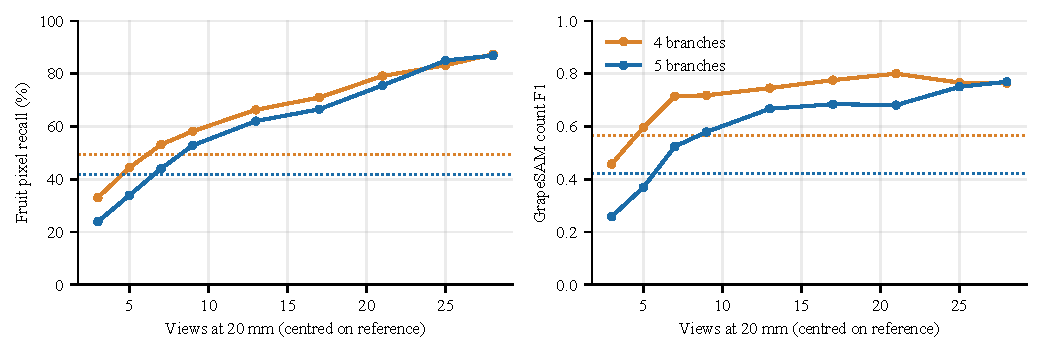
\includegraphics[width=0.9\linewidth]{figures/views_curve.pdf}
\caption{Recall (left) and count F1 (right) against the number of 20~mm views centred on the reference. Dotted lines show the occluded single view. Pixel recall passes the single view at about seven views, count F1 at five to seven.}
\label{fig:views}
\end{figure}

\subsection{How reliable is the evaluation?}
Bootstrap intervals over grapes for the paired gain in count F1 excluded zero at every branch count: $[+0.07, +0.31]$, $[+0.04, +0.39]$, $[+0.18, +0.56]$ and $[+0.20, +0.62]$ for three to six branches. The reconstruction's AP over confidence thresholds (0.69, 0.60, 0.64 and 0.38) also exceeded the single view's (0.39, 0.36, 0.20 and 0.10), so the gain does not depend on the 0.05 threshold. The ranking was unchanged for match radii of 16~px and above; at 8~px every input scored at most 0.42, so detections fall on the right berry but not at its centre.

Perturbing the truth registration by up to 3~px, $1^\circ$ or 1\% changed reconstruction recall by at most 5 points and reconstruction count F1 by at most 0.04, and a 5~px shift by at most 0.08. The measured gains are far larger. The leaf-free count was much less stable: its F1 ranged from 0.67 to 0.91 under the same perturbations, and three-branch reconstructions exceeded it.

Changing the reference view changed the single-view result far more than the reconstruction. At five branches, single-view F1 was $0.38\pm0.18$ across references, against $0.78\pm0.04$ for the reconstruction. Recall was $36\pm8\%$ against $87\pm0\%$. At six branches, two of five references could not be scored.

\textbf{Which grapes are recovered.} Figure~\ref{fig:visibility} relates each labelled grape, 100 instances across the four captures, to the number of aligned views in which its fruit mask covers it. Grapes visible in more than ten views were counted 97\% of the time in the reconstruction, against 55\% in the single view. At 6--10 views the rates were 71\% and 12\%. Grapes seen in at most two views were never recovered, as the three-view rule intends. The reconstruction also counted grapes that were hidden in the reference itself: 4 of 5 such grapes at three branches, 6 of 9 at four, 8 of 12 at five and 7 of 19 at six. At six branches, 7 grapes were not visible in any aligned view.

\begin{figure}[t]
\centering
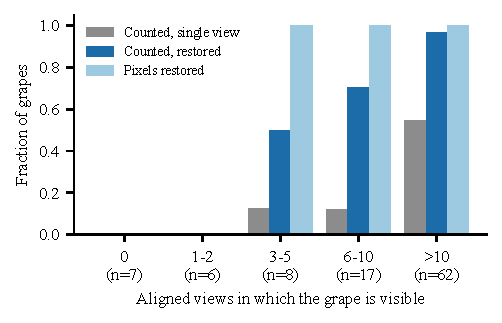
\includegraphics[width=0.9\linewidth]{figures/visibility.pdf}
\caption{Of the 100 labelled grapes (four captures, 20~mm), the fraction counted by GrapeSAM in the single view (grey) and in the reconstruction (dark blue, ``restored'' in the legend), and the fraction whose pixels the reconstruction recovered (light blue), by the number of aligned views in which each grape is visible. Grapes seen in at most two views are never recovered.}
\label{fig:visibility}
\end{figure}

\textbf{Runtime.} For five branches with 28 views at scale 0.8, on a laptop with an RTX~2000 Ada GPU, loading, matching and the joint solve took 16~s and fusion 209~s; SAM~3 masks took 1.5~s per view and GrapeSAM 0.6~s per image. Fusion, tiled NumPy code on the CPU, dominates, so the system currently suits offline analysis only.
